\begin{abstract}
	Processing text documents is crucial in Natural Language Processing; however, computers cannot process text directly in its raw form. To handle this problem, one may use one-hot encoding, which misses a lot of useful information and word relationships from the document. In this work, we explore a powerful word embedding technique called Word2Vec, specifically the Skip-Gram and the Skip-Gram with negative sampling variant, trained on the AG News dataset. We also build a text classification model on top of the word embeddings that achieves an accuracy of 90\%.
\end{abstract}

\section{Introduction}
Natural Language Processing (NLP) is a field of artificial intelligence that focuses on the interaction between computers and human languages. One fundamental task in NLP is transforming raw text into a format that computers can understand and analyze, essential for applications like text classification, sentiment analysis, and machine translation.

One-hot encoding is a simple method to represent text, assigning a unique vector to each word. However, it leads to sparse vectors that fail to capture semantic similarities between words, resulting in a loss of valuable information.

To address these limitations, more sophisticated techniques like word embeddings have been developed. Word embeddings are dense vector representations that capture word meanings by placing similar words closer together in the vector space. One influential technique is Word2Vec, introduced by Mikolov et al., which uses neural networks to learn word associations from large corpora. To see how it works, we discuss some generaly about Skip-Gram and text classification in Section \ref{sec2}, theb we detail our data preparation and implementation in Section \ref{sec3} Finally, we present our results in the Section\ref{sec4}.

\section{Word Embeddings and Skip-Gram Model}\label{sec2}
This section explores word embeddings and the Skip-Gram model,
	a popular method for learning word representations. The Skip-Gram model, proposed by Mikolov et al. \cite{word2vec}. It predicts surrounding context words given a central word. This approach allows the model to learn the semantic meaning of words based on their co-occurrence in text.
   \subsection{Skip-Gram}
   The Skip-Gram model models the word representation by considering a centre word $c$ and predicting $2M$ (can be less) words that are around $c$. The $M$ is referred to as window size, so we have at most $M$ words on the left and $M$ words at the right of the centre words. Figure \ref{fig:skipgram} illustrates a skipgram model with a window size of 2.

   \begin{figure}[H]
	   \begin{subfigure}{0.5\linewidth}
		   \scalebox{0.8}{
			   \tikzstyle{context} = [
	draw = black,
	fill = white,
	minimum size = 0.75cm
	]
			   \tikzstyle{center} = [
	draw = black,
	fill = green!20,
	minimum size = 0.75cm
	]

			   \begin{tikzpicture}[
	node distance = 0cm
	]
				   \node (pts1) at (0,0) {\ldots};
				   \node [context, right=of pts1] (today) {today};
				   \node [context, right=of today] (is) {is};
				   \node [center, right=of is] (a) {a};
				   \node [context, right=of a] (good) {good};
				   \node [context, right=of good] (day) {day};
				   \node [right=of day] (pts2) {\ldots};
				   \path [->,>=latex](a.north) edge [bend left=50 ](good.north);
				   \path [->,>=latex](a.north) edge [bend right=50 ](is.north);
				   \path [->,>=latex](a.north) edge [bend right=50 ](today.north);
				   \path [->,>=latex](a.north) edge [bend left =50](day.north);


				   \node (pts1) at (0,-2) {\ldots};
				   \node [context, right=of pts1] (today) {today};
				   \node [context, right=of today] (is) {is};
				   \node [context, right=of is] (a) {a};
				   \node [center, right=of a] (good) {good};
				   \node [context, right=of good] (day) {day};
				   \node [right=of day] (pts2) {\ldots};
				   \path [->,>=latex](good.north) edge [bend right=50 ](a.north);
				   \path [->,>=latex](good.north) edge [bend right=50 ](is.north);
				   % \path [->,>=latex](good.north) edge [bend right=50 ](today.north);
				   \path [->,>=latex](good.north) edge [bend left =50](day.north);
			   \end{tikzpicture}}
	   \caption{Skip-Gram Illustraion}
	   \end{subfigure}\begin{subfigure}{0.5\linewidth}
		   \scalebox{0.8}{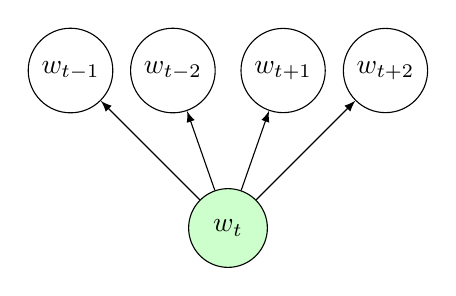
\begin{tikzpicture}[
	node distance = 0.75cm,
	every node/.style = {
	draw = black,
	minimum size = 0.75cm,
	circle
	},
	every edge/.style = {
	-Stealth
	}
	]

			   \node[minimum size=1cm, fill=green!20] (center)  at (0,0) {$w_t$};

			   \node(w1)  at (-2,2) {$w_{t-1}$};
			   \node(w2) at (-0.7,2){$w_{t-2}$};
			   \node(w3) at (0.7, 2) {$w_{t+1}$};
			   \node(w4) at (2,2) {$w_{t+2}$};

			   \draw[->, >=latex] (center) -- (w1);
			   \draw[->, >=latex] (center) -- (w2);
			   \draw[->, >=latex] (center) -- (w3);
			   \draw[->, >=latex] (center) -- (w4);
		   \end{tikzpicture}
   }       \caption{Skip-Gram Model}
	   \end{subfigure}
	   \caption{The skip-gram model}
	   \label{fig:skipgram}
   \end{figure}

   Since, these context words are predicted using the probability $p(w_{t-2}, w_{t-1}, w_{t+1}, w_{t+2} | w_t)$, which is simplified by the following assumption:
   \begin{itemize}
	   \item Each window is an identically and independently distributed sample.
	   \item Within each window, each context word is conditionally independent given the centre word.
	   \item Each context word can be predicted from the centre word in the same way, irrespective of its position.
   \end{itemize}

   Considering the sequence $w_{1:T}$ and a window size $M$, we can derive the negative likelihood of our model written as follows, with the two first assumptions:
   \begin{align}
   J(\mbf{\theta}) &= -\log\prod_{t=1}^{T}P_{\mathbf{\theta}}(w_{t-M:t-1},w_{t+1:t+M}|w_t)\\
   &=-\sum_{t=1}^{T}\sum_{\substack{-M\leq j \leq M,\\ j\neq 0}}\log P_{\mathbf{\theta}}(w_{t+j}|w_t)
   \end{align}
   Where $\mbf{\theta}$ is the parameter of the model. Now, to obtain $P_{\mathbf{\theta}}(w_{t+j}|w_t)$ we consider the third assumption. We also denote the vector representation of a context word $w$ by $\mbf{u}_w$, and $\mbf{v}_w$ for a centre word $w$. Thus, probability for a context words $o$ given a centre word $c$ is given by:
   \begin{equation}
	P_{\mathbf{\theta}}(w_{t+j}=o|w_t=c) = P(o|c) = \frac{e^{\mbf{u}_o^\top\mbf{v}_c}}{\sum_{w\in \mathcal{V}}e^{\mbf{u}_{w}^\top\mbf{v}_c}}
   \end{equation}
   where $\mathcal{V}$ is the set of vocabulary. More generally we have
   \begin{equation}
	\mbf{f_\theta}(w_t=c)=\frac{1}{\sum_{w\in \mathcal{V}}e^{\mbf{u}_{w}^\top\mbf{v}_c}}\begin{bmatrix}
	e^{\mbf{u}_o^\top\mbf{v}_c}\\
	e^{\mbf{u}_o^\top\mbf{v}_c}\\
	\vdots\\
	e^{\mbf{u}_o^\top\mbf{v}_c}\\
	\end{bmatrix}
	= \softmax\left(\mbf{Uv}_c\right)
   \end{equation}
   where $\mbf{f_\theta}(\cdot)$ is our model.

   Furthermore, the parameter of the model can be viewed as two matrices $\mbf{V}$ and $\mbf{U}$, both with a size of $D \times |\mathcal{V}|$. Each column represents the vector embedding of a centre word for $\mbf{V}$, and a context word for $\mbf{U}$. The optimal parameter can be found using the gradient-based optimisation method. After training the model we use $\mbf{V}$ as the embedding and discard $U$.

   One issue with this approach is the computational complexity induced by the softmax when we deal with a large dataset. A solution to this is proposed in \cite{sgns} that we will present in the next section.
   \subsection{Improving skip-gram with negative sampling}
   Before discussing the negative sampling concepts. In the same paper, the author discussed the usage of a subsampling method. This method consists of discarding some frequent words based on a heuristic probability:
   \begin{equation}
	p(w_i) = 1-\sqrt{\frac{t}{f(w_i)}}
   \end{equation}
   Where $f(w_i)$ if the frequency of the word $w_i$, and $t$ a choosen threshold suggested to be $10^{-5}$. By doing this, we reduce the size of our vocabulary while keeping more informative words. However, instead of applying this approach, we will just remove some of the common words known as stopwords from our data for the sake of simplicity.


   On the other hand, the Noise Contrastive Estimation says that a good model should be able to differentiate data from noise by the mean of a binary logistic regression \cite{sgns}. Based on that, for each pair $(c, o)$ (positive) we sample $K$ pairs $(c, w_i)$ (negatives) then, we can create a model that predicts if a given pair is a positive pair or not. This approach yields the following negative log-likelihood for a single pair with the corresponding negative sample.
   \begin{equation}
   J_{c,o}(\mbf{\theta}) = -\log\sigma(\mbf{u}_o^\top\mbf{v}_c) - \sum_{i=1}^{k}\log\sigma(\mbf{u}_{w_i}^\top\mbf{v}_c)
   \end{equation}
   This approach reduces considerably the computational complexity because instead of computing a huge softmax, we compute some simple sigmoid function.


   \subsection{Words embedding evaluation}
   This section discusses how to evaluate word embeddings and how to use them in text classification. A common way to see if the learned embedding makes sense is to see if similar words or related words are located in a specific region of the embedding space (close). This is achieved by computing the $\mathrm{cosine}$ of their embedding vectors. So for two vectors $\mbf{u}$ and $\mbf{v}$ we have:
   \begin{equation}
	\cos(\mbf{u}, \mbf{v}) =\frac{\mbf{u}^\top \mbf{v}}{\|\mbf{u}\|\|\mbf{v}\|}\in [-1,1]
   \end{equation}
   Words with similar meanings will have a cosine similarity close to 1, while dissimilar words will have a value closer to -1. Additionally, the distance between two embeddings is calculated using:
   \begin{equation}
	\mathrm{d}(\mbf{u}, \mbf{v}) = 1 -\cos(\mbf{u}, \mbf{v})\in [0,2]
   \end{equation}

   However, evaluating the overall quality of word embeddings is a complex task. So, in addition the the cosine similarity and distance we can do the following approach:
   \begin{itemize}
	   \item \textbf{Visualization:} techniques like PCA, t-SNE, and UMAP can be used to project word embeddings into a lower-dimensional space for visual inspection. By looking at known similar words and how they cluster together, we can gain insights into the quality of the embeddings.
	   \item \textbf{Extrinsic evaluation:} generally using the words embedding in a downstream task like text classification, or other real-world problems.
	   \item \textbf{Intrinsic evaluation:} This method uses words analogy or asses the correlation with human word similarity judgement.
   \end{itemize}

   As mentioned, a downstream task can be used to evaluate the word embedding, so in the next subsection, we use it for a text classification task.
   \subsection{Text Classification}
   To perform a text classification using the embedded words, we compute the average embedding of the text/sentence:
   \begin{equation}
	\mbf{w}_{\mathrm{sentence}} = \frac{1}{T}\sum_{T}^{t=1}\mbf{w}_t
   \end{equation}
   where $\mbf{w}_t$ is the embedding of the t\textsuperscript{th} word and T is the total number of words.
   Then, we can feed it into a Simple multilayer perceptron to predict the associated class.

   \section{Methodology and implementation}\label{sec3}
   This section presents the implementation of the word2vec model with negative sampling on the AG news dataset. The dataset contains news articles from four classes (World, Sports, Business, and Sci/Tech), with a title and description field for each article. The dataset is split into separate training and test partitions.

   \subsection{Data Preparation}
   The first task is to normalize the text, to be uniform and easy to treat. To achieve that we apply the following process:
   \begin{itemize}
	   \item Split the dataset into three separate files: title, description, and class label.
	   \item Remove common stop words using a list from \cite{stopwords}
	   \item Remove HTML tags that can be handled.
	   \item Replace all numbers (either preceded or followed by letters) with the token $<\mathrm{num}>$.
	   \item Replace all diacritics by their simple form.
	   \item Remove all non-alphanumeric characters by a space.
	   \item Convert all text to lowercase.
	   \item Remove all trailing spaces and multiple spaces.
   \end{itemize}
   We also introduce two special tokens $<\mathrm{unk}>$ to represent an unseen word of the test set and $<\mathrm{pad}>$ to complete a sentence to have the same length in a batch. These two will be useful for the text classification task.

   \subsection{Word2vec Implementation}
   The word2vec model is implemented as a neural network with two layers. The first one represents $\mathbf{V}$ and the second one $\mathbf{U}$, and there is no activation function between these two layers. The softmax function is already included in the \texttt{CrosEntropyLoss} of \texttt{PyTorch} so we do not need to include it.
   We use the module \texttt{nn.Embedding} of \texttt{PyTorch} for $\mbf{V}$ and $\mbf{U}$\footnote{\texttt{nn.Linear} for $\mbf{U}$ with the vanilla Skipgram} to be more efficient instead of using a one-hot vector to extract the corresponding embedding vector. These layers act like a look-up table that maps each index of the words into the corresponding vector representation.

   \subsection{Negative sampling}
   To sample the negative sample follow the suggestion in \cite{sgns}, to use the heuristic probability
   \begin{equation}
	P_n(w) = \frac{U(w)^{3/4}}{Z}
   \end{equation}
   when sampling, where $U$ is the unigram distribution. We do not handle if some of the contexts of the centre word are among the negative sample, as it can be rare, and later re-adjuster when the pair is considered as a positive pair.

   These negative sample are sampled during after constructing the positive pairs, it avoids sampling at each batch which can slow down the training process.
   \subsection{Embedding Visualization}
   For the visualization, we use TensorBoard, which allows us to have an interactive visualization and access to UMAP, t-SNE and PCA for the projection.

   \section{Results and Discussion}\label{sec4}
   After setting the two models and data set, we discuss and present the results of our experimentation in this section.
   \subsection{Words embedding parameter}
   The Table \ref{tab:hyperparameters} list the hyper parameters related to the two words embedding models, where SGNS means Skip-Gram with Negative Sampling.
   \begin{table}[H]
    \centering
    \begin{tabular}{lrr}
        \toprule
        & Skip-gram & SGNS \\
        \midrule
        Window size & 3 & 3 \\
        Negative samples & 10 & N/A \\
        Vocabulary size & 56 465 & 56 465 \\
		Number of words & 1 944 289 & 1 944 289\\
		Number of pairs &4 637 822& 4 637 822\\
		Batch size &4096&4096\\
        Embedding dimension & 256 & 256 \\
        Learning rate & $10^{-3}$ & $10^{-3}$ \\
        Number of iterations & 30 & 5 \\
        Sec./epoch & 60 & 300 \\
        \bottomrule
    \end{tabular}
    \caption{Hyperparameter for the Skip-gram and SGNS models.}
    \label{tab:hyperparameters}
\end{table}
We observe that SGNS is very fast compared to the vanilla skip-gram, due to that fact, we train it for only five epoch.
\begin{figure}[H]\centering
	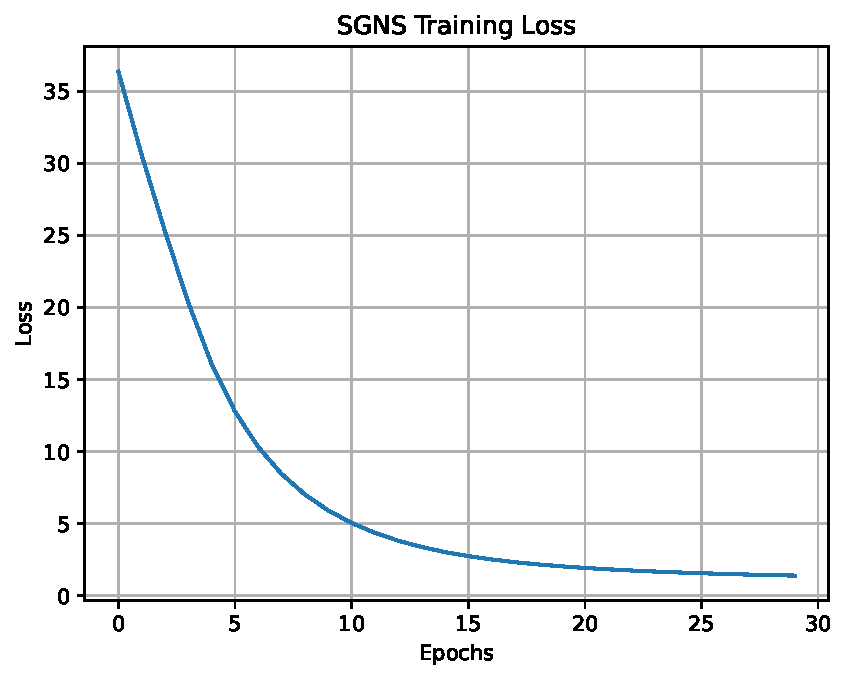
\includegraphics[width=0.45\textwidth]{figures/sgns_loss.pdf}
	\caption{SGNS Loss}
	\label{fig:loss}
\end{figure}
The figure \ref{fig:loss} show the loss function of the SGNS, whis is monotonically decreasing. 
\begin{table}[h]
	\centering
	\begin{minipage}{0.45\linewidth}
		\begin{tabular}{ll}
			\toprule
			\textbf{Word} & \textbf{Similarity} \\
			\midrule
			\multicolumn{2}{c}{\textbf{google}} \\
			\midrule
			search & 0.583 \\
			online & 0.570 \\
			data & 0.544 \\
			internet & 0.525 \\
			\bottomrule
			\multicolumn{2}{c}{\textbf{linux}} \\
			\midrule
			software & 0.600 \\
			internet & 0.582 \\
			technology & 0.557 \\
			products & 0.538 \\
			\bottomrule
			\multicolumn{2}{c}{\textbf{windows}} \\
			\midrule
			software & 0.605 \\
			users & 0.600 \\
			market & 0.548 \\
			search & 0.547 \\
			\bottomrule
			\multicolumn{2}{c}{\textbf{war}} \\
			\midrule
			country & 0.649 \\
			government & 0.626 \\
			iraq & 0.623 \\
			officials & 0.594 \\
			\bottomrule
		\end{tabular}
	\end{minipage}\begin{minipage}{0.45\linewidth}
		\begin{tabular}{ll}
			\toprule
			\textbf{Word} & \textbf{Similarity} \\
			\midrule
			\multicolumn{2}{c}{\textbf{football}} \\
			\midrule
			game & 0.626 \\
			team & 0.595 \\
			players & 0.556 \\
			time & 0.555 \\
			\bottomrule
			\multicolumn{2}{c}{\textbf{food}} \\
			\midrule
			business & 0.392 \\
			giant & 0.383 \\
			industry & 0.380 \\
			customers & 0.372 \\
			\bottomrule
			\multicolumn{2}{c}{\textbf{money}} \\
			\midrule
			business & 0.461 \\
			service & 0.460 \\
			corp & 0.457 \\
			management & 0.453 \\
			\bottomrule
			\multicolumn{2}{c}{\textbf{police}} \\
			\midrule
			killed & 0.627 \\
			military & 0.603 \\
			people & 0.601 \\
			country & 0.597 \\
			\bottomrule
		\end{tabular}
	\end{minipage}
	\caption{Word Similarities}
	\label{tab:word_similarities}
\end{table}


We can effectively observe it the table \ref{tab:word_similarities} that most of these words are related, linked and similar toi the query, whic confirm the effectivenef of our embding method with SGNS. We may also got the similar results with the Vanilla Skip-gram but, due to time and space we are not able to provide the results here.

\begin{figure}[H]\centering
	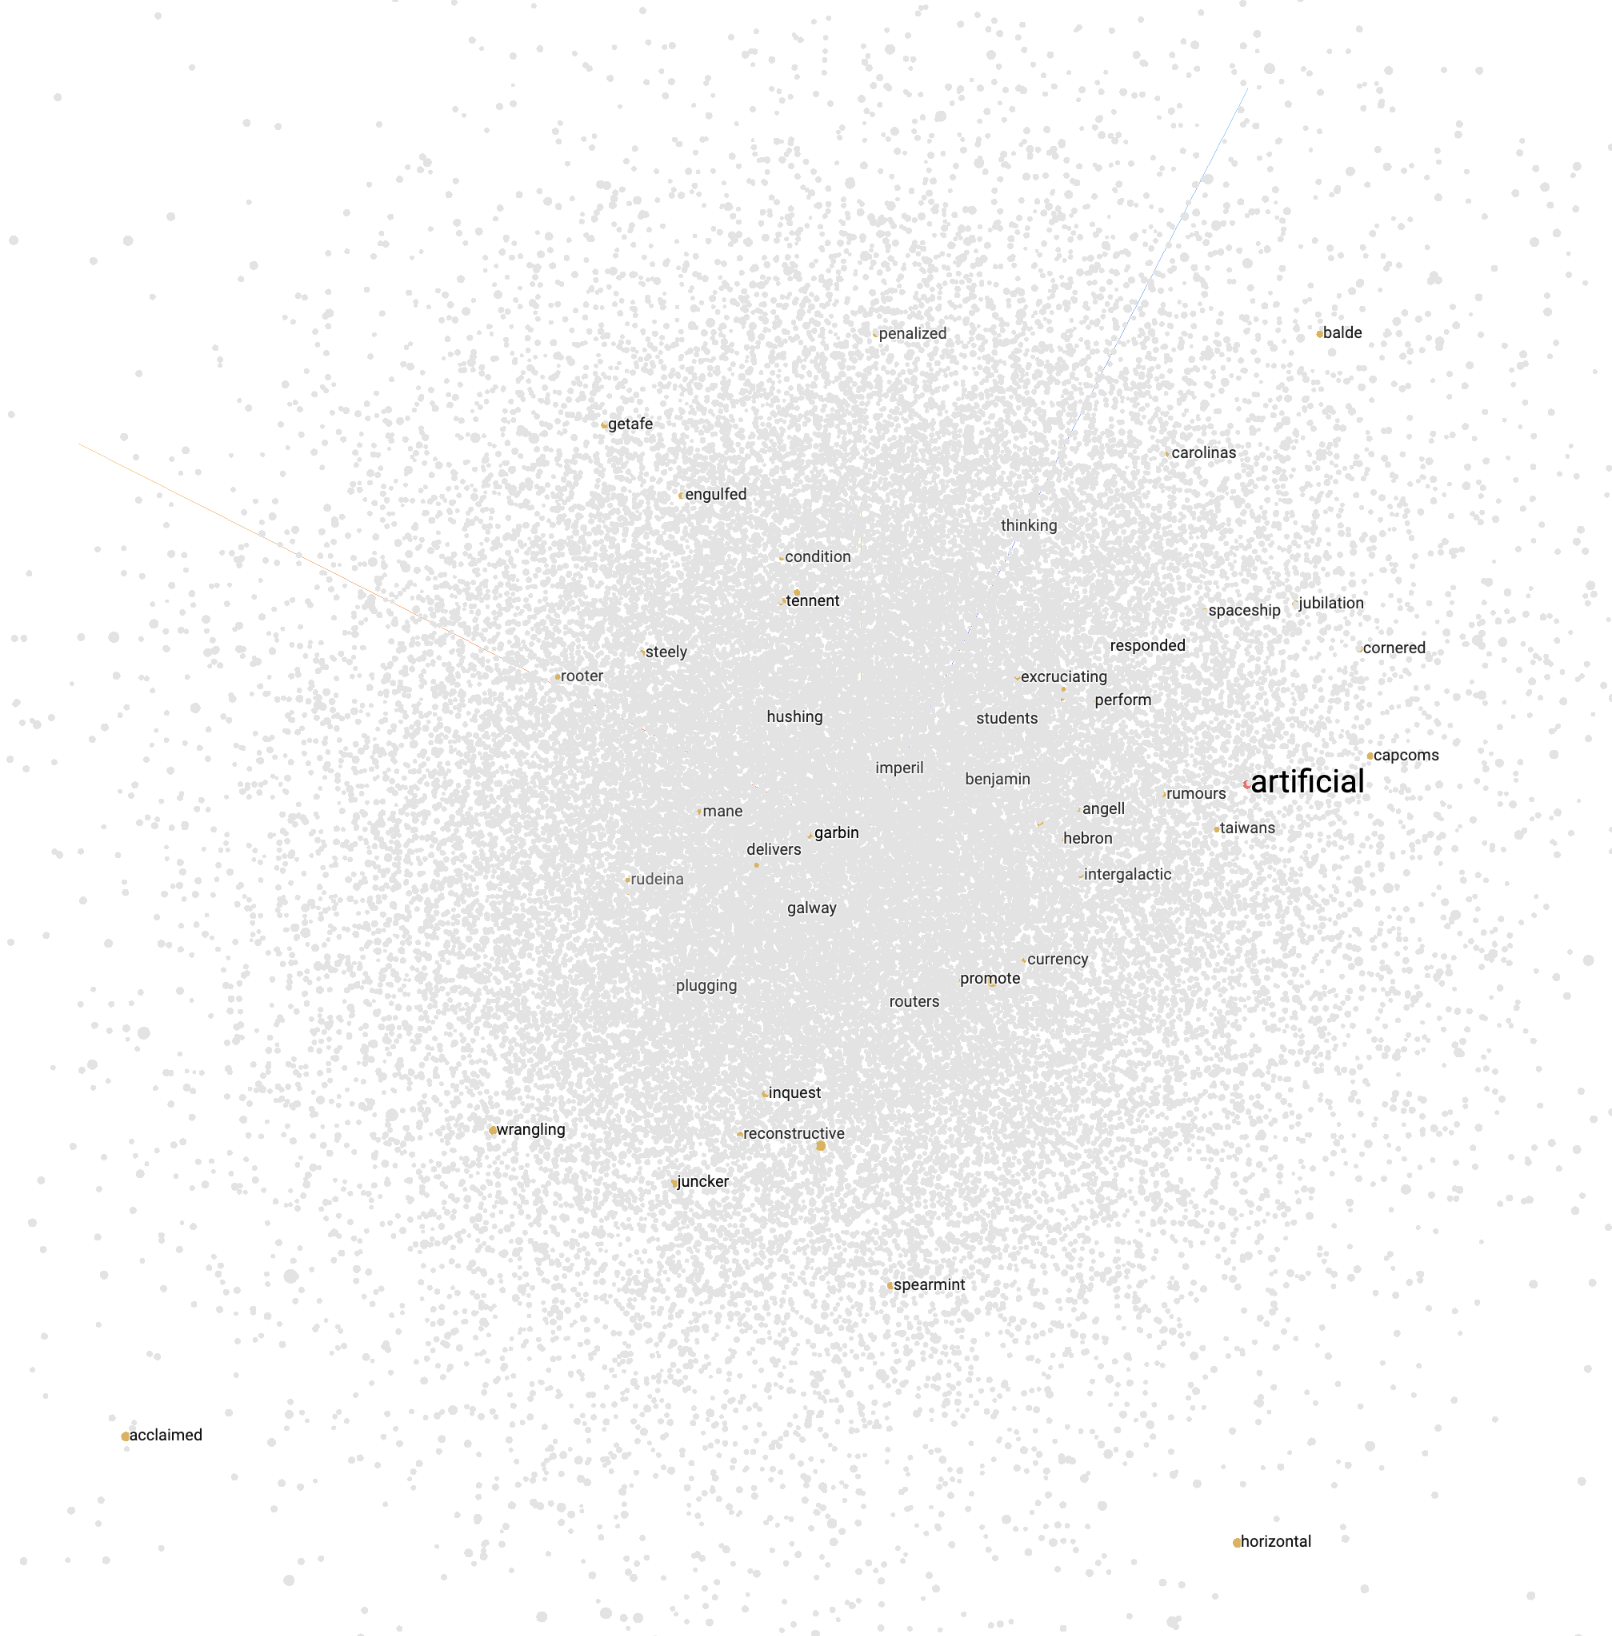
\includegraphics[width=0.45\textwidth]{figures/image.png}
\caption{Tensorboard UMAP visualization}
\label{fig:tboard}
\end{figure}
The Figure \ref{fig:tboard} show a visualization with TensorBoard wher the query is `artificial'.
\subsection{Text classification}
With two layers, we obtain an accuracy of $90\%$ on the test set. The training was fast,
We observe that SGNS is very fast compared to the vanilla skip-gram, due to that fact, we train it for only five epoch, so the results is not yet good enought.

\subsection{Text Classification}
After traingin the text calssifier for 70 epocs, we observe its loss and accuracy in the Figure \ref{fig:loss-acc}.
\begin{figure}[H]\centering
		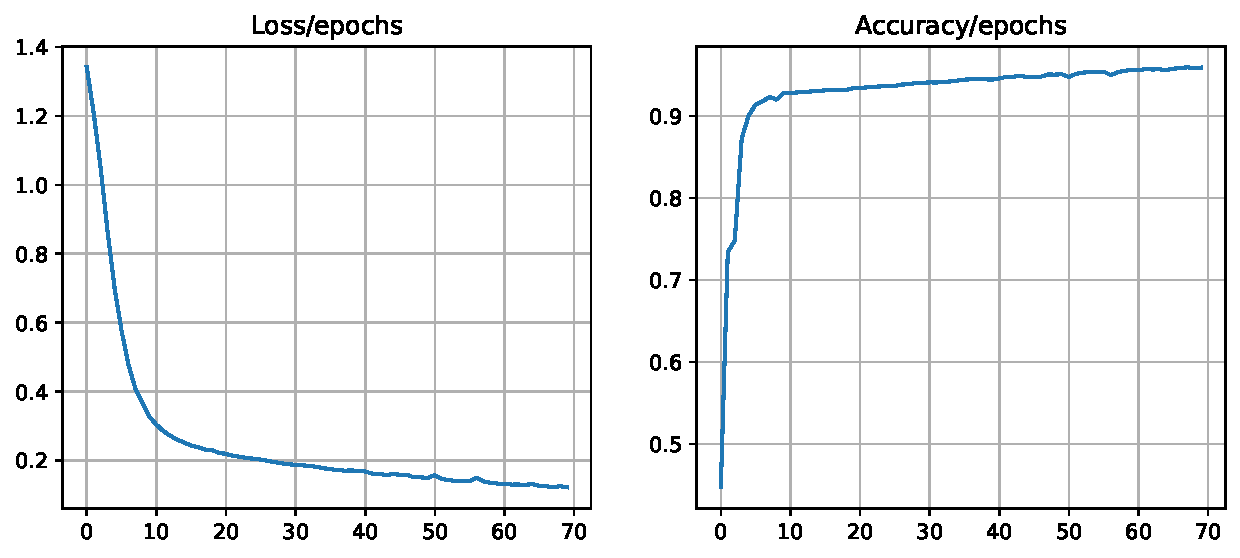
\includegraphics[width=0.45\textwidth]{figures/class_loss.pdf}
	\caption{Loss and accuracy training of the text classiifiers}
	\label{fig:loss-acc}
\end{figure}
On the test set we obtain ana ccuracy of $90\%$, and the Figure \ref{fig:cmat} show it confusion matrix.
\begin{figure}[H]\centering
	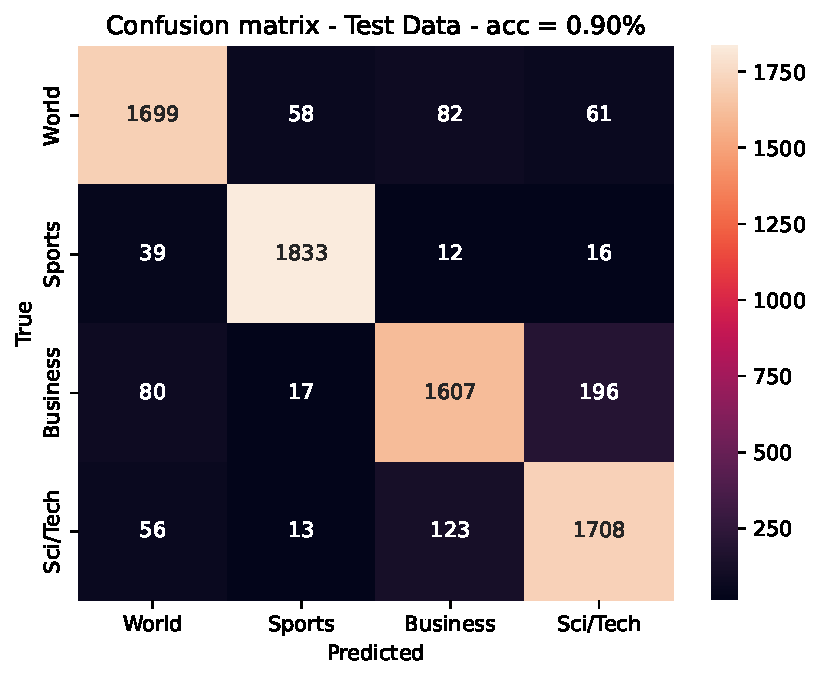
\includegraphics[width=0.45\textwidth]{figures/conf_mat.pdf}
\caption{Confusion matrix of the text classifier on the test set}
\label{fig:cmat}
\end{figure}

We see that it susffer on the Business and Sci/Tech, it may be due to some similarity between thes class.
\section{Conclusion}

   \begin{thebibliography}{1}

	   \bibitem{kamper2022nlp817}
	Herman Kamper. \emph{NLP817}. \href{https://www.kamperh.com/nlp817/}{https://www.kamperh.com/nlp817/}, 2022--2024.

	   \bibitem{word2vec} Mikolov, T., Chen, K., Corrado, G. and Dean, J., 2013. Efficient estimation of word representations in vector space. \textit{arXiv preprint arXiv:1301.3781}.

	   \bibitem{sgns} Mikolov, T., Sutskever, I., Chen, K., Corrado, G.S. and Dean, J., 2013. Distributed representations of words and phrases and their compositionality. \textit{Advances in neural information processing systems, 26}.
	   \bibitem{stopwords} English stopwords list \href{https://github.com/stopwords-iso/stopwords-en/blob/master/stopwords-en.txt}{https://github.com/stopwords-iso/stopwords-en/blob/master/stopwords-en.txt}

	   \bibitem{ang} Andrew Ng, Negative Sampling \href{https://www.youtube.com/watch?v=4PXILCmVK4Q}{https://www.youtube.com/watch?v=4PXILCmVK4Q}
   \end{thebibliography}